\begin{figure}
	\begin{subfigure}{.45\textwidth}
		\centering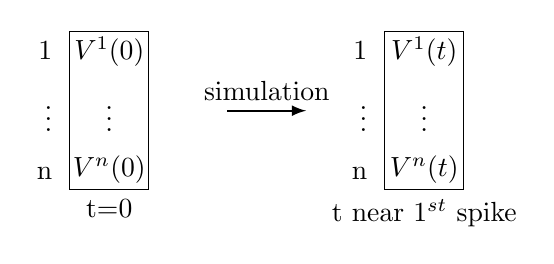
\begin{tikzpicture}[scale=1]
			\draw (0,0) rectangle (1,2);
			\node [below left] at (-.1,2) {1};		\node at (.5,1.75) {$V^1(0)$};
			\node [left] at (-.1,1) {$\vdots$};	\node at (.5,1) {$\vdots$};
			\node [above left] at (-.1,0) {n};		\node at (.5,.25) {$V^n(0)$};
			\node [below] at (.5,0) {t=0};
			
			\draw [thick,-latex] (2,1) -- (3,1) node [midway,above] {simulation};

			\draw (4,0) rectangle (5,2);
			\node [below left] at (3.9,2) {1};		\node at (4.5,1.75) {$V^1(t)$};
			\node [left] at (3.9,1) {$\vdots$};	\node at (4.5,1) {$\vdots$};
			\node [above left] at (3.9,0) {n};		\node at (4.5,.25) {$V^n(t)$};
			\node [below] at (4.5,0) {t near $1^{st}$ spike};
		\end{tikzpicture}
		\caption{Pre-simulation of a network of n neurons}
		\label{}
	\end{subfigure}
	\begin{subfigure}{.45\textwidth}
		\centering\begin{tikzpicture}
			\draw (0,0) -- (0,6) -- (3,6) -- (3,0);
			\node [left] at (0,5.5) {1};	\node at (1.5,5.5) {$\text{\~V}^1(0)=V^1(t)$};
			\node [left] at (0,4.375) {$\vdots$};	\node at (1.5,4.375) {$\vdots$};
			\node [left] at (0,3.25) {n};	\node at (1.5,3.25) {$\text{\~V}^n(0)=V^n(t)$};
			\node [left] at (0,2.75) {n+1};	\node at (1.5,2.75) {$\text{\~V}^{n+1}(0)=V^1(t)$};
			\node [left] at (0,1.625) {$\vdots$};	\node at (1.5,1.625) {$\vdots$};
			\node [left] at (0,.5) {2n};	\node at (1.5,.5) {$\text{\~V}^{2n}(0)=V^n(t)$};
			\node [left] at (0,0) {$\vdots$};	\node at (1.5,0) {$\vdots$};
		\end{tikzpicture}
		\caption{Using the values of potential from the pre-simulation for initializing the greater one}
	\end{subfigure}
	\caption{Initialization procedure}
	\label{fig:inter}
\end{figure}